\begin{exercise}{Propagation dans une chaîne de pendules}{2}{Spé}
{Propagation}{lelay, mines, X}

\begin{questions}
    \questioncours Propagation des OPPH, vitesse de phase, vitesse de groupe.
    \question On considère deux pendules de masse $m$ et de longueur $R$ séparés d'une distance $a$ oscillant dans le même plan avec des angles $\theta_1$ et $\theta_2$. Les deux masses sont reliées entre elles par un ressort de raideur $\kappa$ et de longueur à vide $a$ comme montré dans le schéma ci-dessous.
    \begin{center}
    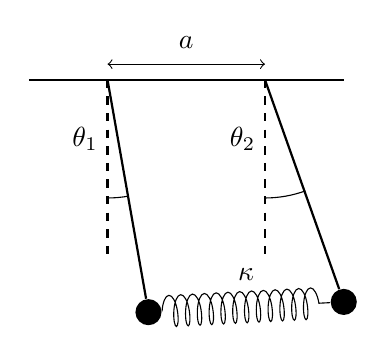
\begin{tikzpicture}
    
    \draw[thick] (-1,0) -- (3,0);
    \draw[<->] (0,0.2) -- (2,0.2);
    \draw (1,0.2) node[above=2pt] {$a$};
    
    \node[circle,fill=black] (a) at (0+0.52,-2.95) {};
    \draw[thick] (0,0) -- (a);
    \draw[thick, dashed] (0,0) -- (0,-2.25);
    \draw (0,-1.5) arc (-90:-80:1.5);
    \draw (0,-0.75) node[anchor=east] {$\theta_1$};
    
    \node[circle,fill=black] (b) at (2+1.0,-2.82) {};
    \draw[thick] (2,0) -- (b);
    \draw[thick, dashed] (2,0) -- (2,-2.25);
    \draw (2,-1.5) arc (-90:-70:1.5);
    \draw (2,-0.75) node[anchor=east] {$\theta_2$};
    
    \draw[decoration={aspect=0.3, segment length=1.5mm, amplitude=2mm,coil},decorate] (a) -- (b);
    \path (a) -- coordinate[midway](m) (b);
    \draw (m) node[above=6pt] {$\kappa$};
    
    \end{tikzpicture}
    \end{center}
    \begin{parts}
        \part Établir l'équation d'évolution de $\theta_1$ et $\theta_2$ au premier ordre. On fera intervenir deux pulsations caractéristique, dont $\omega_0 = \sqrt{\frac{g}{R}}$.
        \part Pour résoudre ce système, on pose $\theta_+ = \theta_1 + \theta_2$ et $\theta_- = \theta_1 - \theta_2$. Réécrire les équations en conséquence.
        \part Pourquoi ce changement de variable était-il intéressant ? Identifier les deux modes de vibration appelés "modes propres" et les décrire qualitativement.
    \end{parts}
    \question On considère maintenant une chaîne de $N \gg 1$ pendules reliés de la même manière, cf schéma ci dessous.
    \begin{center}
    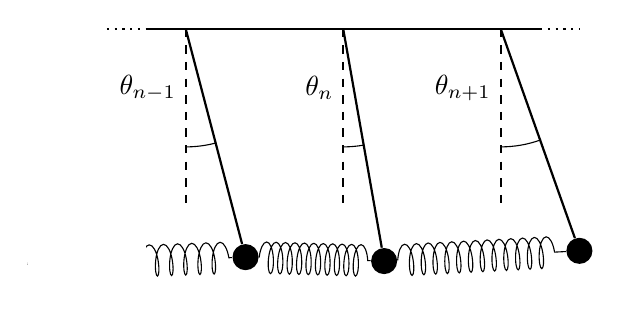
\begin{tikzpicture}
    
    \draw[thick] (-2.5,0) -- (2.5,0);
    \draw[thick, dotted] (-3,0) -- (-2.5,0);
    \draw[thick, dotted] (2.5,0) -- (3,0);
    
    \node[circle,fill=black] (a) at (0+0.52,-2.95) {};
    \draw[thick] (0,0) -- (a);
    \draw[thick, dashed] (0,0) -- (0,-2.25);
    \draw (0,-1.5) arc (-90:-80:1.5);
    \draw (0,-0.75) node[anchor=east] {$\theta_n$};
    
    \node[circle,fill=black] (b) at (2+1.0,-2.82) {};
    \draw[thick] (2,0) -- (b);
    \draw[thick, dashed] (2,0) -- (2,-2.25);
    \draw (2,-1.5) arc (-90:-70:1.5);
    \draw (2,-0.75) node[anchor=east] {$\theta_{n+1}$};
    
    \node[circle,fill=black] (c) at (-2+0.76,-2.90) {};
    \draw[thick] (-2,0) -- (c);
    \draw[thick, dashed] (-2,0) -- (-2,-2.25);
    \draw (-2,-1.5) arc (-90:-75:1.5);
    \draw (-2,-0.75) node[anchor=east] {$\theta_{n-1}$};
    
    \draw[decoration={aspect=0.3, segment length=1.5mm, amplitude=2mm,coil},decorate] (a) -- (b);
    \draw[decoration={aspect=0.3, segment length=1.2mm, amplitude=2mm,coil},decorate] (c) -- (a);
    \draw[decoration={aspect=0.3, segment length=1.8mm, amplitude=2mm,coil},decorate] (-4,-3) -- (c);
    \fill[white] (-4,-2) rectangle (-2.5,-3.5);
    
    \end{tikzpicture}
    \end{center}
    Établir alors l'équation du mouvement du $n$-ième pendule (d'angle $\theta_n$) toujours au premier ordre.
    \question On définit alors $\theta$ tel que $\theta_n(t) = \theta(x = na, t)$. En supposant $a$ petit devant la taille typique des variations spatiales de $\theta$, montrer que $\theta$ vérifie l'équation de Klein-Gordon :
    \begin{align*}
        \pdv[2]{\theta}{t} = c^2 \pdv[2]{\theta}{x} - \omega_0^2\theta
    \end{align*}
    où $c$ est une constante dont on précisera l'expression et la dimension.
    \question On cherche à faire se propager une OPPH dans cette chaîne de pendules. Donnez la relation de dispersion obtenue. On utilisera les variables $\Omega = \omega / \omega_0$ et $K = c k / \omega_0$.
    \question Esquisser l'allure de l'évolution selon $\Omega$ des parties réelles et imaginaires de $K$.
    \question En supposant $\Omega > 1$
    \begin{parts}
        \part Exprimez les vitesses de phase et de groupe adimensionnalisées $V_\varphi$ et $V_g$ en fonction de $\Omega$
        \part Représenter leur allure sur un graphique. Commenter.
    \end{parts}
\end{questions}

\end{exercise}